\clearpage
%\newpage
\section{Preparation}
The preparation phase provides basic information about a target application's performance
characteristics. 
Such information can be obtained by many performance tools.
Currently, we accept performance data generated by both HPCToolkit and GNU gprof.
%Currently, the ROSE-HPCToolKit interface is used to accept performance data generated by HPCToolkit and GNU gprof.
%The interface is used to annotate ROSE AST with performance metrics to
%facilitate building automated performance analysis tools. 
%Detailed information about ROSE-HPCToolKit can be found in Chapter 44 of
%the ROSE tutorial. 
%We only give information relevant to autotuning below.

\subsection{Using HPCToolkit}
%The HPCToolkit~\cite{hpctoolkit} is developed at the Rice University to get
%performance metrics of the target application. 
The HPCToolkit~\cite{hpctoolkit}, developed at the Rice University, is an open source profile-based
performance analysis tool which samples the executions of optimized applications. 
No code
instrumentation is needed to use HPCToolkit. 
But debugging information (by compiling with
the -g option if GCC is used) in the binary executables is needed for the tool to
associate performance metrics with source language constructs.

After installation, a typical session of using HPCToolkit is given below:
{\mySmallFontSize
\begin{verbatim}
% Prepare the executable with debugging information
gcc -g smg2000.c -o smg2000 

% Sample one or more events for the execution, use wall clock here
hpcrun -e WALLCLK -- ./smg2000 -n 120 120 120 -d 3

% Convert the profiling result into a XML format
hpcproftt -p -D /home/liao6/svnrepos/benchmarks/smg2000 ./smg2000 \
  smg2000.WALLCLK.tux268.llnl.gov.10676.0x0 > result.xml

\end{verbatim}
}

\fixme{TODO: update the text when the latest release of HPCToolkit works
on 32-bit platforms}

%A SMG2000~\cite{BrownSemicoarsening2000} (Semicoarsening Multigrid Solver) benchmark from the ASCI Purple
%benchmark suite is chosen to exemplify the use of this system.

Fig.~\ref{fig:hpctoolkitSmg2000} shows the profiling results of SMG2000
using HPCToolkit. 
A statement in a loop takes more than 46\% execution time, which makes the
loop dominant, most expensive loop of the entire program.
\begin{figure}[htbp]  
	\centering
		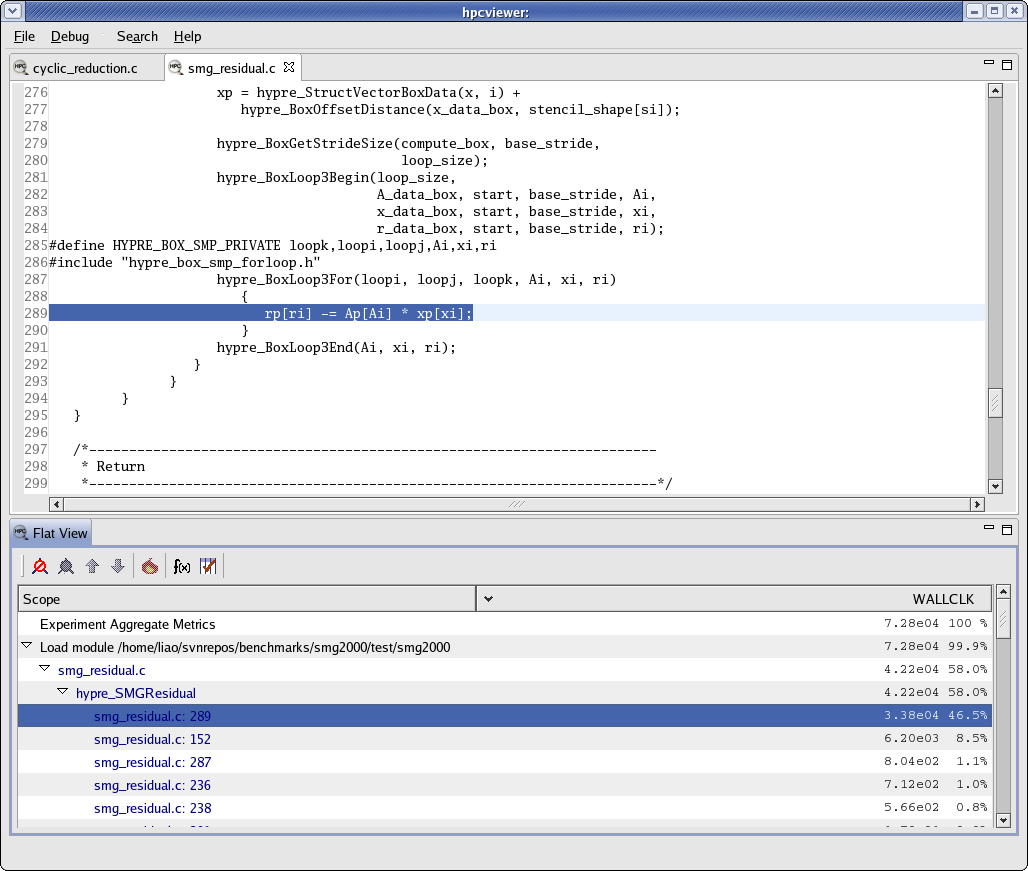
\includegraphics[width=0.9\textwidth]{hpctoolkit-smg2000.png}
	\caption{Profiling results of SMG2000 using HPCToolkit}
	\label{fig:hpctoolkitSmg2000}
\end{figure}

\subsection{Using gprof}
GNU gprof can generate line-by-line performance information for an
application. A typical session to generate such information is given below:
\begin{verbatim}
[liao@codes]$ gcc -g seq-pi.c -pg
[liao@codes]$ ./a.out
[liao@codes]$ gprof -l -L a.out gmon.out &>profile.result
\end{verbatim}

The option {\tt -l} tells gprof to output line-by-line profiling
information. 
{\tt -L} causes gprof to output full file path information, which is needed
for ROSE to accurately match performance data to source code.

An excerpt of an output file for smg2000 looks like the following:
{\scriptsize
\begin{verbatim}
Flat profile:

Each sample counts as 0.01 seconds.
  %   cumulative   self     
 time   seconds   seconds     name
 35.01     13.08    13.08     hypre_SMGResidual (/home/liao/smg2000/struct_ls/smg_residual.c:289 @ 804caa4)
  9.05     16.46     3.38     hypre_CyclicReduction (/home/liao/smg2000/struct_ls/cyclic_reduction.c:1130 @ 8054af4)
  8.40     19.60     3.14     hypre_SMGResidual (/home/liao/benchmarks/smg2000/struct_ls/smg_residual.c:291 @ 804cab9)
  7.67     22.46     2.87     hypre_CyclicReduction (/home/liao/smg2000/struct_ls/cyclic_reduction.c:910 @ 8053191)
  5.97     24.70     2.23     hypre_CyclicReduction (/home/liao/smg2000/struct_ls/cyclic_reduction.c:998 @ 8053a28)
  5.27     26.66     1.97     hypre_SMGResidual (/home/liao/smg2000/struct_ls/smg_residual.c:238 @ 804d129)
  2.86     27.73     1.07     hypre_SMGResidual (/home/liao/smg2000/struct_ls/smg_residual.c:287 @ 804cacb)
  2.28     28.59     0.85     hypre_CyclicReduction (/home/liaosmg2000/struct_ls/cyclic_reduction.c:853 @ 8052bae)
  2.07     29.36     0.78     hypre_CyclicReduction (/home/liao/smg2000/struct_ls/cyclic_reduction.c:1061 @ 8054450)
  1.79     30.03     0.67     hypre_SemiRestrict (/home/liao/smg2000/struct_ls/semi_restrict.c:262 @ 8056a8c)
  1.67     30.66     0.62     hypre_SemiInterp (/home/liao/smg2000/struct_ls/semi_interp.c:294 @ 8055d6c)
  1.12     31.07     0.42     hypre_CyclicReduction (/home/liao/smg2000/struct_ls/cyclic_reduction.c:1133 @ 8054b2f)
  0.96     31.43     0.36     hypre_CyclicReduction (/home/liao/smg2000/struct_ls/cyclic_reduction.c:912 @ 80531a6)
  0.87     31.76     0.33     hypre_StructAxpy (/home/liao/smg2000/struct_mv/struct_axpy.c:69 @ 806642c)
  0.80     32.06     0.30     hypre_CyclicReduction (/home/liao/smg2000/struct_ls/cyclic_reduction.c:1002 @ 8053a60)
  0.78     32.35     0.29     hypre_SMGResidual (/home/liao/smg2000/struct_ls/smg_residual.c:236 @ 804d14b)
  0.72     32.62     0.27     hypre_CyclicReduction (/home/liao/smg2000/struct_ls/cyclic_reduction.c:1063 @ 8054462)
  0.60     32.84     0.23     hypre_SMGAxpy (/home/liao/smg2000/struct_ls/smg_axpy.c:69 @ 8064970)
  0.59     33.06     0.22     hypre_CycRedSetupCoarseOp (/home/liao/smg2000/struct_ls/cyclic_reduction.c:369 @ 8051149)
  0.59     33.28     0.22     hypre_SMGResidual (/home/liao/smg2000/struct_ls/smg_residual.c:240 @ 804d146)
  0.51     33.48     0.19     hypre_StructVectorSetConstantValues (/home/liao/smg2000/struct_mv/struct_vector.c:578 @ 806fedc)
  0.48     33.66     0.18     hypre_SMGSetupInterpOp (/home/liao/smg2000/struct_ls/smg_setup_interp.c:292 @ 804ea04)
  0.46     33.83     0.17     hypre_SemiInterp (/home/liao/smg2000/struct_ls/semi_interp.c:227 @ 80556e8)
  0.40     33.98     0.15     hypre_CyclicReduction (/home/liao/smg2000/struct_ls/cyclic_reduction.c:855 @ 8052bd4)
  0.40     34.12     0.15     hypre_StructMatrixInitializeData (/home/liao/smg2000/struct_mv/struct_matrix.c:359 @ 80678b0)
  ...
\end{verbatim}
}



%We use the self seconds associated with each source line and attach them to
%ROSE AST as AST attributes named WALLCLK.

